\ifdefined\ishandout
  \documentclass[handout,landscape]{beamer} 
\else
  \documentclass[landscape]{beamer}
\fi

%\hypersetup{pdfpagemode=FullScreen} %Enabling this option will cause the slides to go full-screen on opening

\mode<handout>
{
  \usepackage{pgf}
  \usepackage{pgfpages}

\pgfpagesdeclarelayout{6 on 1 boxed}
{
  \edef\pgfpageoptionheight{\the\paperheight} 
  \edef\pgfpageoptionwidth{\the\paperwidth}
  \edef\pgfpageoptionborder{0pt}
}
{
  \pgfpagesphysicalpageoptions
  {%
    logical pages=6,%
    physical height=\pgfpageoptionheight,%
    physical width=\pgfpageoptionwidth%
  }
  \pgfpageslogicalpageoptions{1}
  {%
    border code=\pgfsetlinewidth{2pt}\pgfstroke,%
    border shrink=\pgfpageoptionborder,%
    resized width=.5\pgfphysicalwidth,%
    resized height=.5\pgfphysicalheight,%
    center=\pgfpoint{.25\pgfphysicalwidth}{.833\pgfphysicalheight}%
  }%
  \pgfpageslogicalpageoptions{2}
  {%
    border code=\pgfsetlinewidth{2pt}\pgfstroke,%
    border shrink=\pgfpageoptionborder,%
    resized width=.5\pgfphysicalwidth,%
    resized height=.5\pgfphysicalheight,%
    center=\pgfpoint{.75\pgfphysicalwidth}{.833\pgfphysicalheight}%
  }%
  \pgfpageslogicalpageoptions{3}
  {%
    border code=\pgfsetlinewidth{2pt}\pgfstroke,%
    border shrink=\pgfpageoptionborder,%
    resized width=.5\pgfphysicalwidth,%
    resized height=.5\pgfphysicalheight,%
    center=\pgfpoint{.25\pgfphysicalwidth}{.5\pgfphysicalheight}%
  }%
  \pgfpageslogicalpageoptions{4}
  {%
    border code=\pgfsetlinewidth{2pt}\pgfstroke,%
    border shrink=\pgfpageoptionborder,%
    resized width=.5\pgfphysicalwidth,%
    resized height=.5\pgfphysicalheight,%
    center=\pgfpoint{.75\pgfphysicalwidth}{.5\pgfphysicalheight}%
  }%
  \pgfpageslogicalpageoptions{5}
  {%
    border code=\pgfsetlinewidth{2pt}\pgfstroke,%
    border shrink=\pgfpageoptionborder,%
    resized width=.5\pgfphysicalwidth,%
    resized height=.5\pgfphysicalheight,%
    center=\pgfpoint{.25\pgfphysicalwidth}{.167\pgfphysicalheight}%
  }%
  \pgfpageslogicalpageoptions{6}
  {%
    border code=\pgfsetlinewidth{2pt}\pgfstroke,%
    border shrink=\pgfpageoptionborder,%
    resized width=.5\pgfphysicalwidth,%
    resized height=.5\pgfphysicalheight,%
    center=\pgfpoint{.75\pgfphysicalwidth}{.167\pgfphysicalheight}%
  }%
}


  \pgfpagesuselayout{6 on 1 boxed}[letterpaper, border shrink=5mm]
  \nofiles
}

\usepackage{listings}
\usepackage{multimedia}
\usepackage[normalem]{ulem}
\usepackage{ifthen}

\usetheme{Warsaw} 
\usecolortheme{seahorse}
\useoutertheme{infolines} 

\setbeamertemplate{blocks}[rounded][shadow=true] 

\author{Joe Fields}
\title{Introduction to Proof} 

\date{Lecture 27 (GIAM \S 5.3) \newline divisibility statements and other proofs using PMI}
\institute[SCSU]{ {\tt fieldsj1@southernct.edu} }

\newcommand{\versionNum}{$3.2$\ }

\newboolean{InTextBook}
\setboolean{InTextBook}{false}
\newboolean{InWorkBook}
\setboolean{InWorkBook}{false}
\newboolean{InHints}
\setboolean{InHints}{false}

%When this boolean is true (beginning in Section 5.1) we will use the convention
% that $0 \in \Naturals$.  If it is false we will continue to count $1$ as the smallest
%natural number (thus making Giuseppe Peano spin in his grave...)
 
\newboolean{ZeroInNaturals}

%This boolean is used to distinguish the version where we use $\sim$ rather than $\lnot$

\newboolean{LNotIsSim}

%The values of the last two booleans are set in ``switches.tex''

\setboolean{ZeroInNaturals}{true}
\setboolean{LNotIsSim}{false}


\let\savedlnot\lnot
\ifthenelse{\boolean{LNotIsSim}}{\renewcommand{\lnot}{\sim} }{}

%This command puts different amounts of space depending on whether we are
% in the text, the workbook or the hints & solutions manual. 
\newcommand{\twsvspace}[3]{%
 \ifthenelse{\boolean{InTextBook} }{\vspace{#1}}{%
  \ifthenelse{\boolean{InWorkBook} }{\vspace{#2}}{%
   \ifthenelse{\boolean{InHints} }{\vspace{#3}}{} %
   }%
  }%
 }


\newcommand{\wbvfill}{\ifthenelse{\boolean{InWorkBook}}{\vfill}{}}
\newcommand{\wbitemsep}{\ifthenelse{\boolean{InWorkBook} }{\rule[-24pt]{0pt}{60pt}}{}}
\newcommand{\textbookpagebreak}{\ifthenelse{\boolean{InTextBook}}{\newpage}{}}
\newcommand{\workbookpagebreak}{\ifthenelse{\boolean{InWorkBook}}{\newpage}{}}
\newcommand{\hintspagebreak}{\ifthenelse{\boolean{InHints}}{\newpage}{}}

\newcommand{\hint}[1]{\ifthenelse{\boolean{InHints}}{ {\par \hspace{12pt} \color[rgb]{0,0,1} #1 } }{}}
\newcommand{\inlinehint}[1]{\ifthenelse{\boolean{InHints}}{ { \color[rgb]{0,0,1} #1 } }{}}

\newlength{\cwidth}
\newcommand{\cents}{\settowidth{\cwidth}{c}%
\divide\cwidth by2
\advance\cwidth by-.1pt
c\kern-\cwidth
\vrule width .1pt depth.2ex height1.2ex
\kern\cwidth}

\newcommand{\sageprompt}{ {\tt sage$>$} }
\newcommand{\tab}{\rule{20pt}{0pt}}
\newcommand{\blnk}{\rule{1.5pt}{0pt}\rule{.4pt}{1.2pt}\rule{9pt}{.4pt}\rule{.4pt}{1.2pt}\rule{1.5pt}{0pt}}
\newcommand{\suchthat}{\; \rule[-3pt]{.5pt}{13pt} \;}
\newcommand{\divides}{\!\mid\!}
\newcommand{\tdiv}{\; \mbox{div} \;}
\newcommand{\restrict}[2]{#1 \,\rule[-4pt]{.25pt}{14pt}_{\,#2}}
\newcommand{\lcm}[2]{\mbox{lcm} (#1, #2)}
\renewcommand{\gcd}[2]{\mbox{gcd} (#1, #2)}
\newcommand{\Naturals}{{\mathbb N}}
\newcommand{\Integers}{{\mathbb Z}}
\newcommand{\Znoneg}{{\mathbb Z}^{\mbox{\tiny noneg}}}
\ifthenelse{\boolean{ZeroInNaturals}}{%
  \newcommand{\Zplus}{{\mathbb Z}^+} }{%
  \newcommand{\Zplus}{{\mathbb N}} }
\newcommand{\Enoneg}{{\mathbb E}^{\mbox{\tiny noneg}}}
\newcommand{\Qnoneg}{{\mathbb Q}^{\mbox{\tiny noneg}}}
\newcommand{\Rnoneg}{{\mathbb R}^{\mbox{\tiny noneg}}}
\newcommand{\Rationals}{{\mathbb Q}}
\newcommand{\Reals}{{\mathbb R}}
\newcommand{\Complexes}{{\mathbb C}}
%\newcommand{\F2}{{\mathbb F}_{2}}
\newcommand{\relQ}{\mbox{\textsf Q}}
\newcommand{\relR}{\mbox{\textsf R}}
\newcommand{\nrelR}{\mbox{\raisebox{1pt}{$\not$}\rule{1pt}{0pt}{\textsf R}}}
\newcommand{\relS}{\mbox{\textsf S}}
\newcommand{\relA}{\mbox{\textsf A}}
\newcommand{\Dom}[1]{\mbox{Dom}(#1)}
\newcommand{\Cod}[1]{\mbox{Cod}(#1)}
\newcommand{\Rng}[1]{\mbox{Rng}(#1)}

\DeclareMathOperator\caret{\raisebox{1ex}{$\scriptstyle\wedge$}}

\newtheorem*{defi}{Definition}
\newtheorem*{exer}{Exercise}
\newtheorem{thm}{Theorem}[section]
\newtheorem*{thm*}{Theorem}
\newtheorem{lem}[thm]{Lemma}
\newtheorem*{lem*}{Lemma}
\newtheorem{cor}{Corollary}
\newtheorem{conj}{Conjecture}

\renewenvironment{proof}%
{\begin{quote} \emph{Proof:} }%
{\rule{0pt}{0pt} \newline \rule{0pt}{15pt} \hfill Q.E.D. \end{quote}}


\newcommand{\vs}{\rule{0pt}{12pt}}
\newcommand{\notimplies}{\;\not\!\!\!\implies}
\newcommand{\dx}{\,\mbox{d}x}

\AtBeginSection[]
{
 \begin{frame}{Table of Contents} 
  \tableofcontents[currentsection]
 \end{frame}
}

%%%% SAVE %%%%
%{ %magic to get a full screen image...
%\setbeamertemplate{navigation symbols}{}  % hide navigation buttons 
%\setbeamertemplate{background canvas}{\centerline{\includegraphics 
%	[height=\paperheight]{Cantor_4.jpeg}}}
%\begin{frame}[plain]
%\rule{0pt}{0pt}
%\end{frame} 
%} %end of magic


\begin{document}

\begin{frame}[plain]
  \titlepage
\end{frame}

\section{intro}

\begin{frame}{Pierre de Fermat}
\begin{itemize}
\item The ``prince of amateurs'' \pause
\item Most famous for Fermat's Last Theorem ($a^n + b^n = c^n$ has no non-trivial solutions when $n>2$.) \pause
\item Finally proved (after a bit more than 300 years!) by Andrew Wiles. \pause
\end{itemize}
\end{frame}


{ %magic to get a full screen image...
\setbeamertemplate{navigation symbols}{}  % hide navigation buttons 
\setbeamertemplate{background canvas}{\centerline{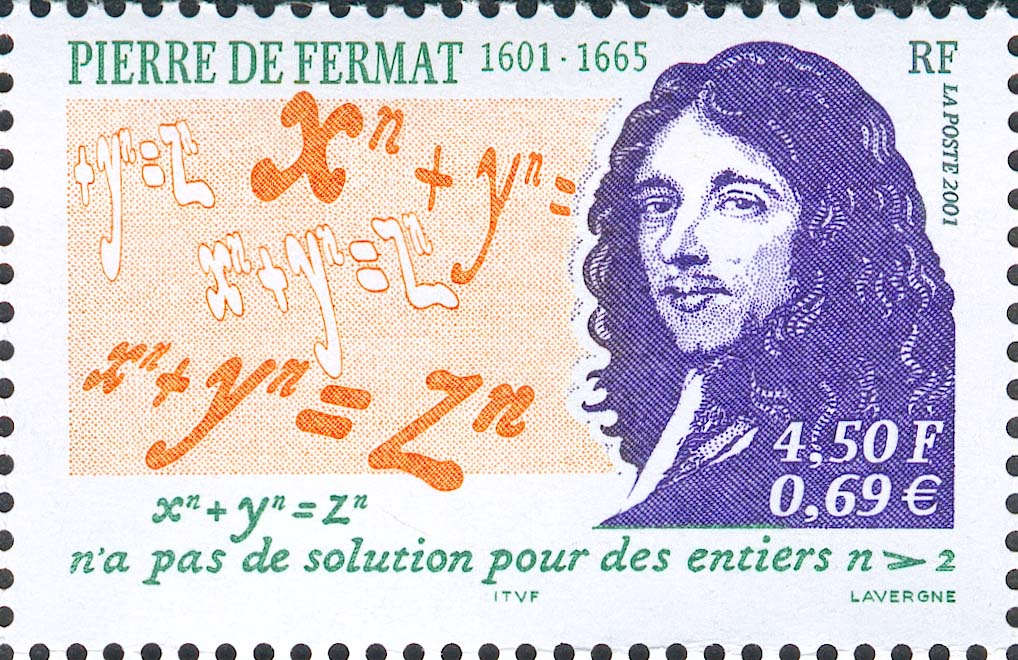
\includegraphics 
	[height=\paperheight]{fermat1.jpg}}}
\begin{frame}[plain]
\rule{0pt}{0pt}
\end{frame} 
} %end of magic

{ %magic to get a full screen image...
\setbeamertemplate{navigation symbols}{}  % hide navigation buttons 
\setbeamertemplate{background canvas}{\centerline{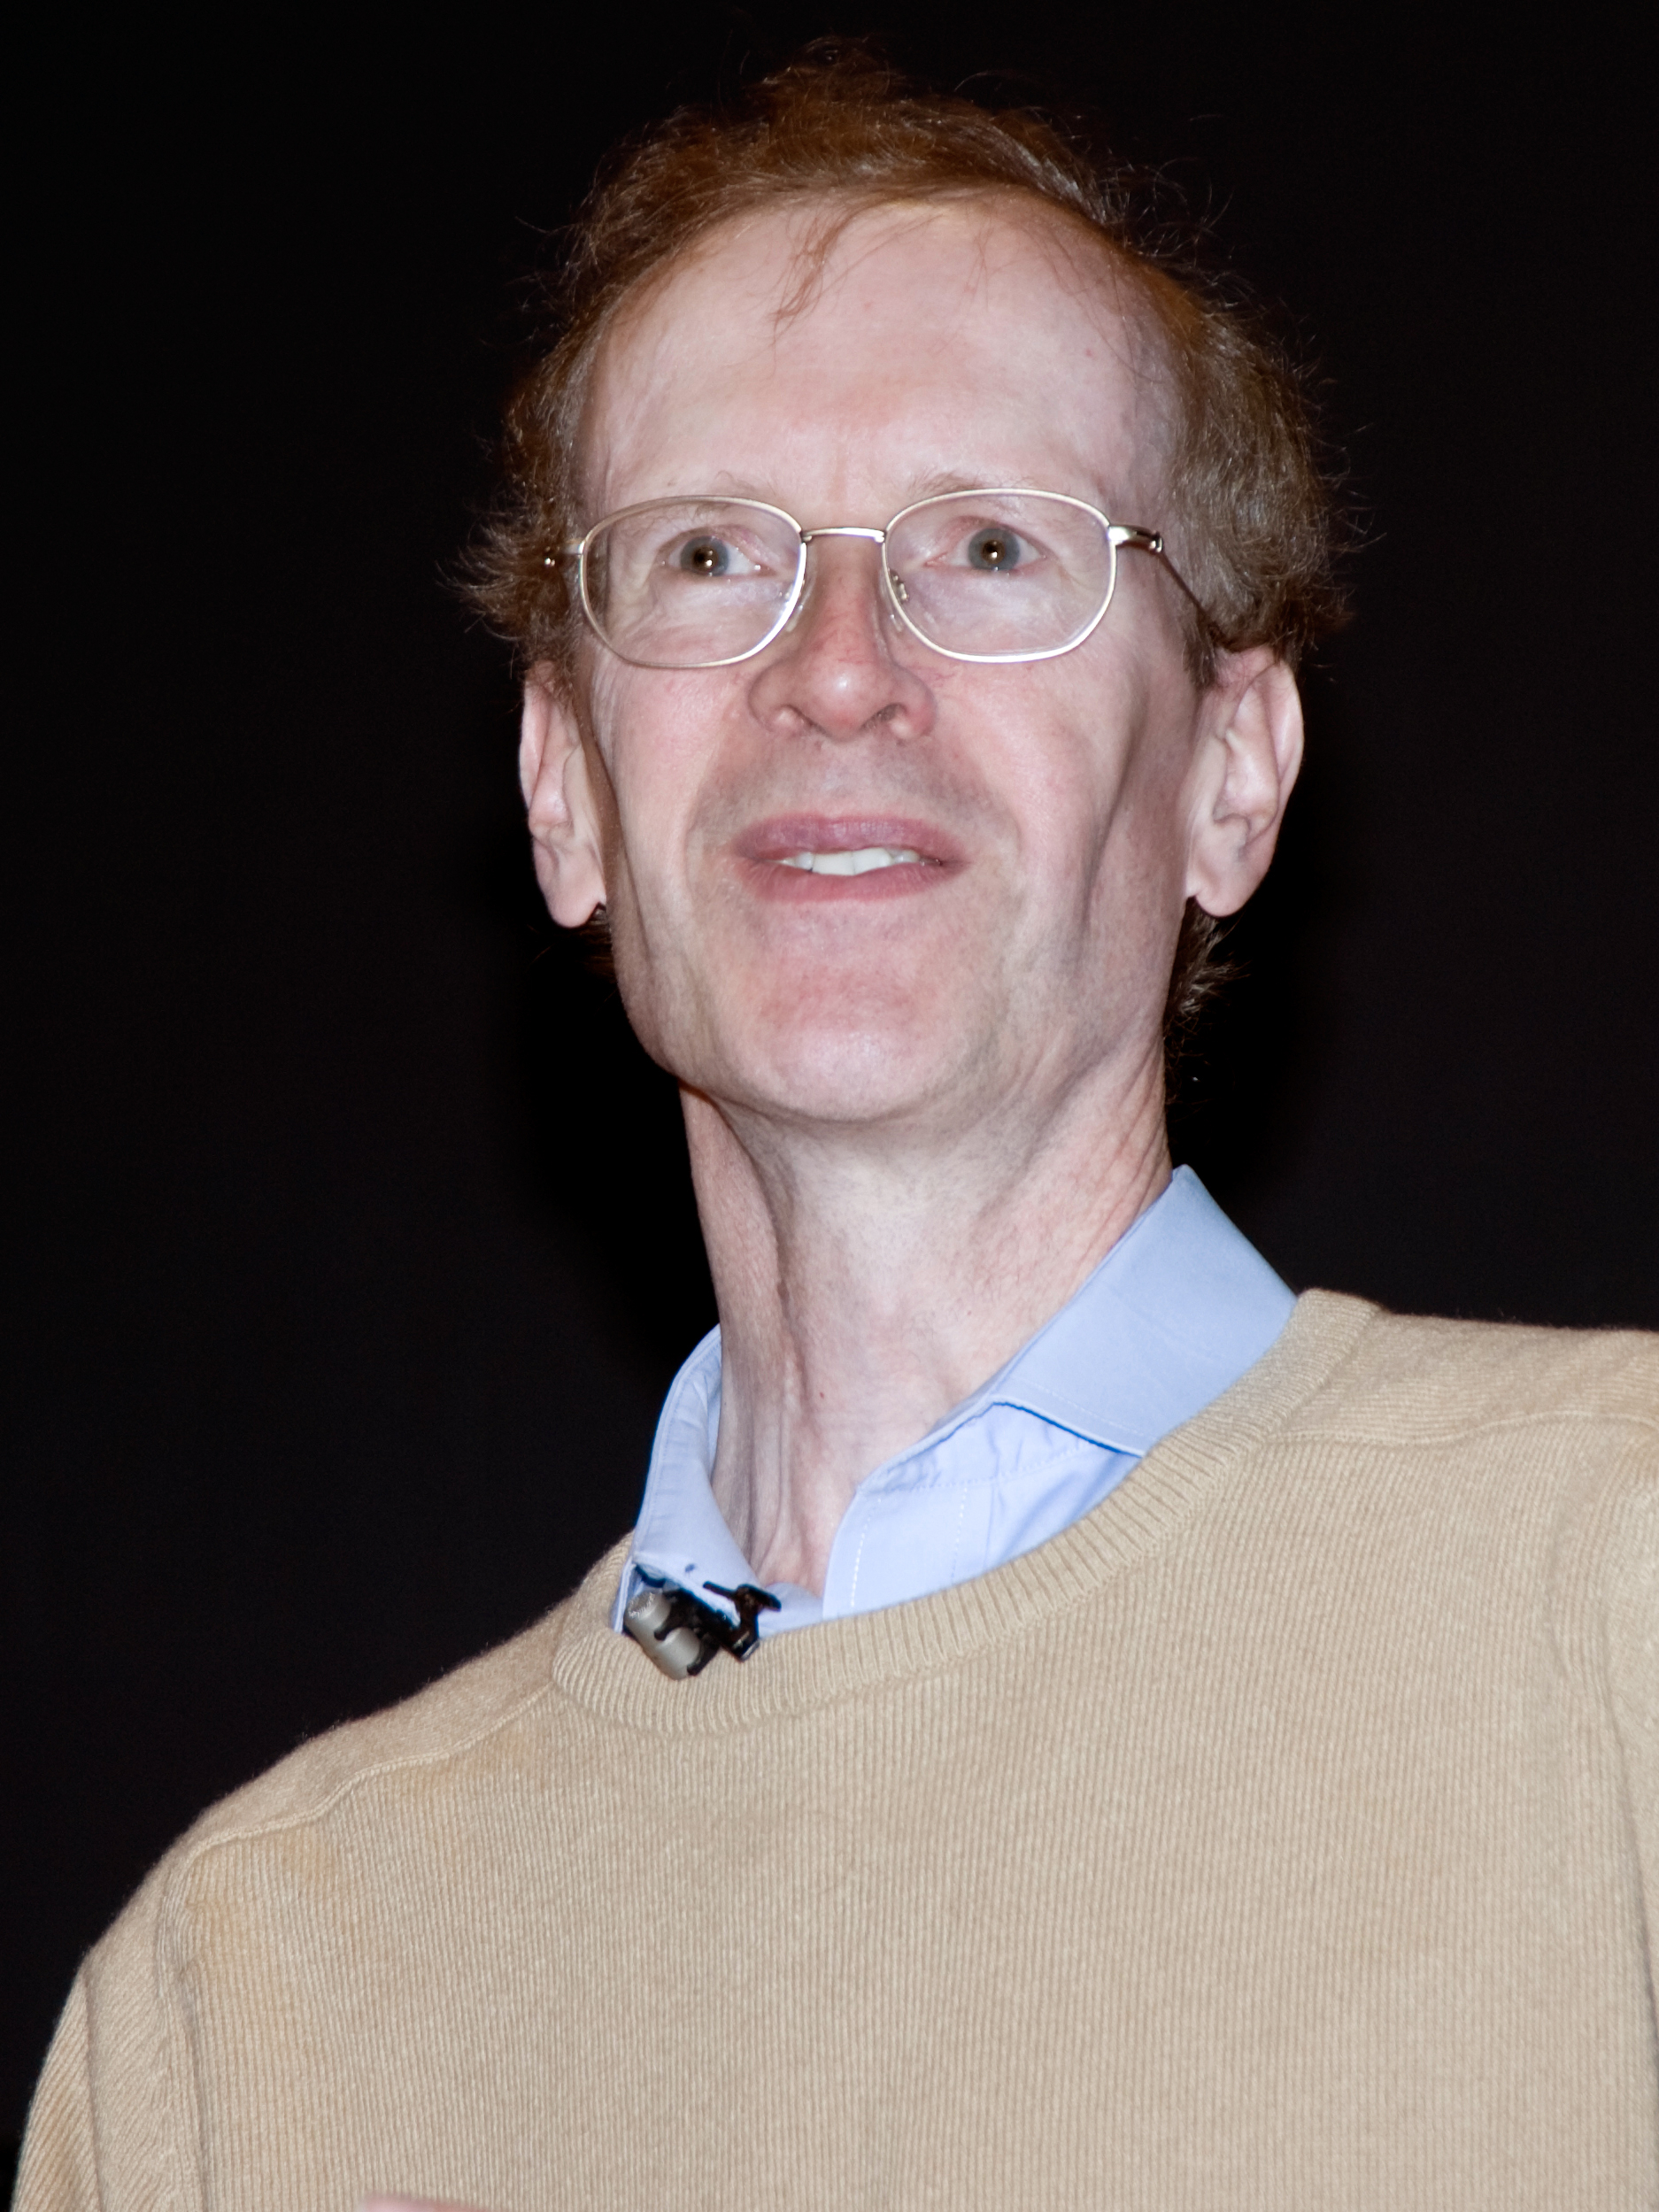
\includegraphics 
	[height=\paperheight]{Wiles.jpg}}}
\begin{frame}[plain]
\rule{0pt}{0pt}
\end{frame} 
} %end of magic

\section{flt}

\begin{frame}{Fermat's little theorem}
\begin{itemize}
\item Fermat definitely proved this one! \pause
\item It's about $p$-th powers $\mod p$ (when $p$ is a prime.) \pause 

\begin{thm*}
If $p$ is a prime, then for all integers $x$, $x^p \mod p \; = \; x \mod p$.
\end{thm*}

\pause

\item We can also write this as $x^p \equiv x \pmod{p}$ or as $p \divides (x^p - x)$
\end{itemize}

\end{frame}

\begin{frame}{why}
\begin{itemize}
\item One way to see that FLT is true is to look at the binomial coefficients of the form $\binom{p}{k}$ (where $p$ is prime):
\[ \binom{p}{k} \; = \; \frac{ p! }{k! (p-k)!} . \] \pause
\item The only ones where that $p$ in the numerator could get cancelled is when $k=p$, or when $k=0$ (so $p-k = p$). \pause
\item In other words all the binomial coefficients in a prime row of Pascal's triangle will be divisible by that prime (except for the 1's on either end). \pause
\end{itemize}

\end{frame}

\begin{frame}{example}
\begin{itemize}

\item As an example, notice how all the numbers (other than the first and the last) in the 5th row are divisible by $5$? \pause \newline

\begin{tabular}{ccccccccccc}
\rule{6pt}{0pt} 1 \rule{6pt}{0pt}& &\rule{6pt}{0pt} 5 \rule{6pt}{0pt}& & \rule{6pt}{0pt}10\rule{6pt}{0pt} & & \rule{6pt}{0pt}10 \rule{6pt}{0pt}& & \rule{6pt}{0pt}5\rule{6pt}{0pt} & & \rule{6pt}{0pt}1\rule{6pt}{0pt} \\
\end{tabular}
\pause

\vspace{.2in}

\item If we expand $(x+1)^5$ we get $x^5 + 5x^4 + 10x^3 + 10x^2 + 5x +1$. \pause
\item Because all the stuff in the middle of that expansion is divisible by $5$, it follows that
\[ (x+1)^5 \equiv x^5 + 1 \pmod{5}. \] 
\end{itemize}
\end{frame}

\section{examples}

\begin{frame}{divisibility proofs}
\begin{itemize}
\item There are a lot of divisibility statements that are really FLT with a thing disguise.
\item For instance, since FLT tells us that $3 \divides x^3 - x$ we can add something that is clearly divisible by 3, like $3x+3$ to get $3 \divides x^3 + 2x + 3$.\pause
\item I'm giving you a ``peek behind the curtain here.'' \pause
\item We'll prove such statements by induction.
\end{itemize}
\end{frame}

\begin{frame}{pmi in a divisibility proof}
\begin{thm*}
\[ \forall x \in \Naturals, \quad 3 \divides x^3 + 2x + 3. \]
\end{thm*}

\pause
{\em Proof:} (By induction on $x$.) \pause

{\bf Basis:} When $x=0$, $x^3 + 2x + 3 \; = \; 3$ and clearly $3 \divides 3$.

\pause

{\bf Inductive step:} Suppose that $x \in \Naturals$ is given and $3 \divides x^3 + 2x + 3$.  We want to show
that $3 \divides (x+1)^3 + 2(x+1) + 3$.  

\end{frame}

\begin{frame}{continued}

Note that 
\begin{align*}
 \uncover<1->{(x+1)^3 +2(x+1) + 3 \; & = \; (x^3 + 3x^2 + 3x + 1) + (2x + 2) + 3 \\}
 \uncover<2->{                      & = \; (x^3 + 2x + 3) + 3x^2 + 3x + 1 +  2  \\}
 \uncover<3->{                       & = \; (x^3 + 2x + 3) + 3(x^2 + x + 1)  \\}
\end{align*}
\uncover<4->{
By the inductive hypothesis and the definition of divisibility, we know that $x^3 + 2x + 3 = 3m$ for some integer $m$.} 

\uncover<5->{
It follows that $(x+1)^3 +2(x+1) + 3 \; = \; 3 \cdot (m + x^2 + x + 1)$.}

\uncover<6->{Thus $3 \divides (x+1)^3 + 2(x+1) + 3$ because $(m + x^2 + x + 1)$ is an integer.}

\uncover<7->{ \hfill {\em Q.E.D.} }

\end{frame}

\begin{frame}{another standard trick}
\begin{itemize}
\item If we're working modulo $n$, numbers like $n+1$ or $2n+1$ are equivalent to $1$.  Since $1$ to any power is $1$, we can simplify certain expressions. \pause
\item For example $6^n \pmod{5} \equiv 1$.  Equivalently, $5 \divides (6^n - 1)$ for any $n\in \Naturals$. \pause
\item Again, that was a look at how we cook up such problems. We'll prove them using induction.
\end{itemize}
\end{frame}

\begin{frame}{example 2}
\begin{thm*}
\[ \forall n\in \Naturals, \; 5 \divides 6^n-1. \]
\end{thm*}

\pause
{\em Proof:} (By induction on $n$.) \pause

{\bf Basis:} When $n=0$ we have $6^0-1 = 0$.  Note that $5 \divides 0$ is true. \pause

{\bf Inductive step:} Suppose $k$ is a particular but arbitrary natural number such that $5 \divides 6^k-1 $.
We want to show that $5 \divides 6^{k+1}-1 $.
\end{frame}

\begin{frame}{continued}
Notice that $6^{k+1}-1 \; = \; 6 \cdot 6^k -1 \; = \; (5+1) \cdot 6^k -1 \; = \; 5 \cdot 6^k + (6^k - 1)$.
\pause

By the inductive hypothesis we know that $5 \divides (6^k - 1)$ so there is an integer $m$ such that $6^k - 1 = 5m$.
\pause

Thus, $6^{k+1}-1 \; = \; 5 \cdot 6^k + 5m \; = \; 5 \cdot (6^k + m)$. \pause Since $6^k + m$ is an integer this shows that
$5 \divides 6^{k+1}-1$ as desired.
\pause 

\hfill {\em Q.E.D.} 
\end{frame}

\begin{frame}{inequalities}
\begin{itemize}
\item Inequalities are another category of statements that can often be proved using induction.\pause
\item Which is bigger, $2^n$ or $n!$? \pause
\item Let's check it out on the calculator.\pause
\end{itemize}

\begin{thm*} 
\[ \forall n \geq 4 \in \Naturals, 2^n < n! \]
\end{thm*}

\end{frame}

\begin{frame}{prove an inequality}
\begin{proof} (By mathematical induction)

\noindent {\bf Basis:} When $n=4$ we have $2^4 < 4!$, which is certainly 
true ($16 < 24$). \pause

\noindent {\bf Inductive step:} Suppose that $k$ is a natural number 
with $k > 4$, and that $2^k < k!$.  \pause Multiply the left hand side of this
inequality by $2$ and the right hand side by $k+1$ to get \pause

\[ 2\cdot 2^{k} < (k+1) \cdot k!. \]

\noindent So

\[ 2^{k+1} < (k+1)!. \]

\end{proof}
\end{frame}

\begin{frame}{one last example}
\begin{thm*}
For all $n \in \Naturals$, if $n \geq 3$ then $2n+1 \leq n^2$.
\end{thm*}
\pause

{\em Proof:} (By induction on $n$.) \pause

\noindent {\bf Basis:} When $n=3$, $2n+1 = 7$ and $n^2 = 9$. Clearly $7 \leq 9$. \pause

\noindent {\bf Inductive step:} Suppose that $k$ is a natural number 
with $k \geq 3$, and that $2k+1 \leq k^2$. \pause Note that since $k \geq 3$, $2 \leq 2k+1$. \pause
Adding the two inequalities ( $2k+1 \leq k^2$ and $2 \leq 2k+1$) gives $2k+3 \leq k^2 + 2k + 1$. \pause

So $2(k+1)+1 \leq (k+1)^2$ which is the inductive conclusion. \pause

\hfill {\em Q.E.D} 

\end{frame}



\end{document}
